% Origin: written by Claude (AI) - first draft of the Milestone 1 report. See ai_usage.md, Section 5.
\documentclass[11pt,a4paper]{article}
\usepackage[utf8]{inputenc}
\usepackage[T1]{fontenc}
\usepackage{lmodern}
\usepackage[margin=2.2cm]{geometry}
\usepackage{amsmath,amssymb}
\usepackage{booktabs}
\usepackage{graphicx}
\usepackage{caption}
\captionsetup{font=small}
\usepackage[compact]{titlesec}
\usepackage[hidelinks]{hyperref}
\usepackage{microtype}
\setlength{\parskip}{4pt}
\setlength{\parindent}{0pt}

\newcommand{\cvrpd}{\mbox{CVRP-D}}
\newcommand{\tspd}{\mbox{TSP-D}}
\newcommand{\hc}{\mbox{HamCycle}}
\newcommand{\bp}{\mbox{BinPacking}}
\newcommand{\feas}{\mbox{CVRP-Feas}}

% generated by src/m1_values.py - do not edit by hand
\newcommand{\IsPlaceholder}{0}
\newcommand{\TeamSeed}{19409}
\newcommand{\SeedFormula}{4445 + 5096 + 3185 + 6683}
\newcommand{\SeedModeText}{the last four digits of each ID are read as one four-digit number and these numbers are added}
\newcommand{\InstanceName}{MediDrone-s19409}
\newcommand{\InstanceFile}{instances/medidrone\_s19409.vrp}
\newcommand{\NumClusters}{4}
\newcommand{\NumEU}{52}
\newcommand{\NumAS}{48}
\newcommand{\NumRandom}{20}
\newcommand{\NumClustered}{80}
\newcommand{\ClusterSizes}{20, 20, 20, 20}
\newcommand{\TotalDemand}{1629}
\newcommand{\LowerBoundK}{17}
\newcommand{\FleetK}{18}
\newcommand{\FFDK}{17}
\newcommand{\Triples}{1{,}030{,}301}
\newcommand{\RuleViolations}{0}
\newcommand{\NeutralViolations}{3{,}416}
\newcommand{\NeutralMax}{150.0}
\newcommand{\PythonVersion}{3.13.18}
\newcommand{\MemberRows}{Kubilay Karaca & 2364445 & 4445 \\
Tuana Pektaş & 2365096 & 5096 \\
Elif Ozan & 2483185 & 3185 \\
Zehra Gebeş & 2366683 & 6683 \\}


\begin{document}

\begin{center}
{\small CMP 3005 -- Analysis of Algorithms \textperiodcentered{} Fall 2026--2027}\\[2pt]
{\Large\bfseries Term Project -- Milestone 1: Theory \& Data}\\[2pt]
{\large MediDrone Istanbul -- Capacitated Vehicle Routing Problem}\\[6pt]
\begin{tabular}{lll}
\toprule
\textbf{Member} & \textbf{Student ID} & \textbf{Last four digits}\\
\midrule
\MemberRows
\bottomrule
\end{tabular}
\end{center}

%=====================================================================
\section{Problem definitions}

\textbf{CVRP.} We are given a complete undirected graph $G=(V,E)$ with
$V=\{0,1,\dots,n\}$, where vertex $0$ is the depot (central lab) and $1,\dots,n$ are the
customers (clinics); a distance function $d:E\to\mathbb{R}^{+}$ that satisfies the
triangle inequality; a demand $q_i\in\mathbb{Z}^{+}$ with $q_i\le Q$ for every customer;
a vehicle capacity $Q\in\mathbb{Z}^{+}$ and a fleet of $K$ identical vehicles. A
\emph{feasible solution} is a set of at most $K$ routes such that every route starts and
ends at the depot, every customer is visited by exactly one route exactly once, and the
total demand on every route is at most $Q$.
\begin{itemize}
\item \textbf{Optimisation version:} find a feasible solution of minimum total distance.
\item \textbf{Decision version (\cvrpd):} given $(G,d,q,Q,K)$ and a bound
$B\in\mathbb{R}^{+}$, is there a feasible solution with total distance at most $B$?
\end{itemize}

\textbf{Problems used in the reductions.}
\begin{itemize}
\item \textbf{\hc:} does an undirected graph $H=(V_H,E_H)$ with $N\ge3$ vertices contain a
cycle that visits every vertex exactly once? (NP-complete, Karp 1972.)
\item \textbf{\tspd:} given a complete graph on $N$ vertices with weights $w$ that satisfy
the triangle inequality and a bound $B$, is there a Hamiltonian cycle (tour) of total
weight at most $B$?
\item \textbf{\feas:} given demands $q_1,\dots,q_n$, a capacity $Q$ and $K$ vehicles (distances
ignored), can all customers be served with at most $K$ vehicles of capacity $Q$?
\item \textbf{\bp:} given item sizes $s_1,\dots,s_n\in\mathbb{Z}^{+}$, a bin capacity $C$ and a
number $k$, can the items be packed into at most $k$ bins of capacity $C$? (NP-complete,
Garey \& Johnson 1979.)
\end{itemize}

%=====================================================================
\section{Reduction sketches}

\subsection{\texorpdfstring{Step A: \hc{} $\le_p$ \tspd}{Step A: HamCycle to TSP-D}}
\textbf{Construction.} Given $H=(V_H,E_H)$, build the complete graph on the same $N$
vertices with
\[
w(u,v)=\begin{cases}1 & \text{if } \{u,v\}\in E_H,\\ 2 & \text{otherwise,}\end{cases}
\qquad B=N .
\]
\textbf{Polynomial time.} There are $N(N-1)/2$ weights to write, so the construction takes
$O(N^2)$ time. The weights satisfy the triangle inequality: one edge weighs at most $2$
and two edges together weigh at least $2$.

\textbf{($\Rightarrow$)} If $H$ has a Hamiltonian cycle, it uses $N$ edges of $E_H$; as a
tour it weighs exactly $N\le B$.\\
\textbf{($\Leftarrow$)} A tour has exactly $N$ edges of weight at least $1$, so it weighs at
least $N$. If it weighs at most $B=N$, all its edges have weight $1$, i.e.\ all are edges
of $H$, so the tour is a Hamiltonian cycle of $H$.

\subsection{\texorpdfstring{Step B: \tspd{} $\le_p$ \cvrpd}{Step B: TSP-D to CVRP-D}}
\textbf{Construction.} Given a \tspd{} instance on vertices $v_0,\dots,v_{N-1}$ with
weights $w$ and bound $B$, let $v_0$ be the depot and $v_1,\dots,v_{N-1}$ the customers
($n=N-1$), keep $d=w$ and the same $B$, and choose
\[
q_i=1\ \ (i=1,\dots,n),\qquad Q=n,\qquad K=1 .
\]
One vehicle can carry all demand, but only one vehicle exists, so the CVRP instance is
``really'' a TSP instance. The instance is valid ($q_i\le Q$, $d$ satisfies the triangle
inequality) and is built in $O(N^2)$ time.

\textbf{($\Rightarrow$)} A tour of weight at most $B$, read starting from $v_0$, is one route
$(0,c_1,\dots,c_n,0)$ that visits every customer once, carries $n\le Q$ and uses
$1\le K$ vehicle; its distance equals the tour weight, so it is at most $B$.\\
\textbf{($\Leftarrow$)} With $K=1$, a feasible solution is a single route that starts at
the depot, visits every customer exactly once and returns -- a Hamiltonian cycle on all
$N$ vertices with the same weight, at most $B$.

\subsection{Composition}
Let $f$ (Step A) run in time $p(|x|)$ and $g$ (Step B) in time $r(|y|)$, where $p$ and $r$
are polynomials. A procedure that runs for $p(|x|)$ steps writes at most $p(|x|)$ symbols,
so $|f(x)|\le p(|x|)$ and $g(f(x))$ is computed in time $p(|x|)+r(p(|x|))$. A polynomial
of a polynomial is again a polynomial, so $g\circ f$ runs in polynomial time. It is
correct because $x\in\hc \iff f(x)\in\tspd \iff g(f(x))\in\cvrpd$. Hence
$\hc\le_p\cvrpd$. Since \hc{} is NP-complete, a polynomial-time algorithm for \cvrpd{}
would decide \hc{} in polynomial time; therefore \cvrpd{} is NP-hard.

\subsection{\texorpdfstring{\bp{} $\le_p$ \feas}{BinPacking to CVRP-Feas}}
\textbf{Key observation.} A feasible solution exists if and only if the customers can be
split into at most $K$ groups, each with total demand at most $Q$. ($\Rightarrow$) The
customer sets of the routes are such groups. ($\Leftarrow$) Each group can be served by
one route $0\to\dots\to0$ in any order, because $G$ is complete.

\textbf{Construction.} Given a \bp{} instance $(s_1,\dots,s_n;\,C;\,k)$, set
\[
q_i=s_i\ \ (i=1,\dots,n),\qquad Q=C,\qquad K=k .
\]
If some $s_i>C$, the answer is trivially NO; output a fixed NO instance instead (two
customers with $q=1$, $Q=1$, $K=1$). The mapping takes $O(n)$ time.

\textbf{Correctness.} Bins correspond to vehicles and items to customers, so a packing
into at most $k$ bins of capacity $C$ is exactly a split of the customers into at most
$K$ groups with load at most $Q$. By the key observation: YES for \bp{} $\iff$ YES for
\feas. Hence \feas{} is NP-hard.

%=====================================================================
\section{Seed calculation}
The seed is the sum of the last four digits of all team members' student IDs (table
above):
\[
\text{seed}=\SeedFormula=\mathbf{\TeamSeed}.
\]

%=====================================================================
\begin{minipage}{\linewidth}
\section{Our MediDrone instance}
\centering
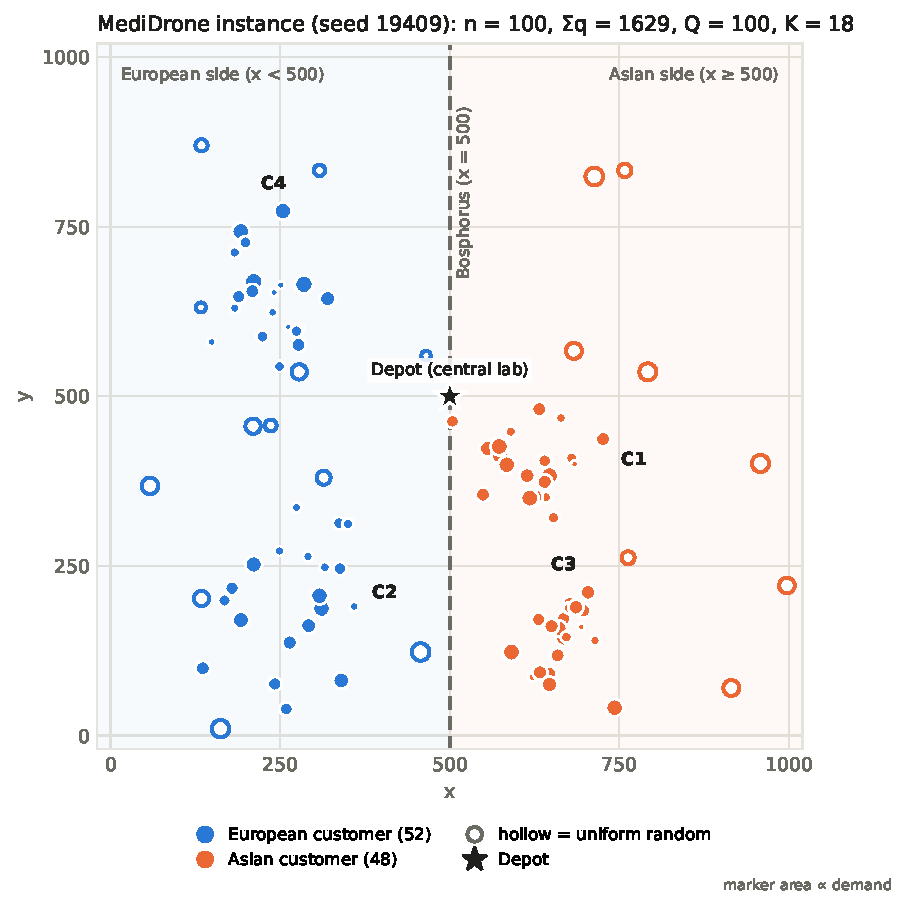
\includegraphics[width=0.8\linewidth]{../../figures/medidrone_instance.pdf}
\captionof{figure}{MediDrone instance generated with seed \TeamSeed. The depot is at $(500,500)$ in
the $1000\times1000$ square; the Bosphorus at $x=500$ splits it into the European
($x<500$) and Asian ($x\ge500$) sides. There are $n=100$ customers: \NumClustered{} in
\NumClusters{} clusters on both sides and \NumRandom{} uniformly random (hollow
markers). Demands are integers in $[1,30]$ (marker area $\propto$ demand),
$\sum q_i=\TotalDemand$, $Q=100$, $K=\lceil \TotalDemand/100\rceil+1=\FleetK$. Distance:
$d(i,j)=$ Euclidean distance $+\,150$ if $i$ and $j$ lie on different sides.}
\end{minipage}

{\small\textbf{References.} R.\,M.~Karp, ``Reducibility among combinatorial problems'',
1972. \textperiodcentered{} M.\,R.~Garey, D.\,S.~Johnson, \emph{Computers and
Intractability: A Guide to the Theory of NP-Completeness}, 1979.}

\end{document}
